\documentclass{article}

% Formatting
\usepackage[utf8]{inputenc}
\usepackage[margin=1in]{geometry}
\usepackage[titletoc,title]{appendix}
\usepackage[spanish]{babel}
\usepackage{amsmath,amsfonts,amssymb,mathtools}
\usepackage{graphicx,float}
\usepackage[ruled,vlined]{algorithm2e}
\usepackage{algorithmic}
\usepackage{minted}
\usemintedstyle{borland}
\usepackage{subcaption}
\usepackage{multicol}
\usepackage{listings}
\usepackage{xcolor}
\usepackage{biblatex}
\addbibresource{ref.bib}
\usepackage{minted}



% Title content
\title{Práctica 5 método Monte Carlo}
\author{Denisse Leyva}
\date{Marzo 18, 2021}

\begin{document}

\maketitle




% Introduction
\section{Introducción}
El método Monte Carlo es idóneo para situaciones en las cuales algún valor o alguna distribución no se conoce y resulta complicado de determinar de manera analítica. Siguiendo los ejemplos de Kurt \cite{Will_Kurt} paralelicemos algunos casos sencillos en esta práctica.
Supongamos que se ocupa conocer el valor de una integral que no se nos antoja resolver para nada, como, por ejemplo

\[ \int_{3}^{7} f(x) \,dx \] para
\[f(x) = \frac {1}{exp(x) + exp(-x)}\]
Por suerte, 2$f(x)/ \pi$ es una función de distribución valida, ya que
\[ \int_{-\infty}^{\infty}\frac{2}{\pi} f(x) \,dx = 1\]
Este hecho nos permite generar números pseudoaleatorios con la distribución 	g(x) = 2 f(x)/ $\pi$, \\ así \ estimar \[ \int_{3}^{7} g(x) \,dx \]
\ y de ahí normalizar el estimado para que sea \[\int_{3}^{7} f(x) \,dx\] \\
Se puede comparar con el resultado aproximado de Wolfram Alpha, 0.048834, para llegar a una satisfacción que no estemos completamente mal. Se debe notar que cada ejecución dará un resultado distinto ya que es una muestra pseudoaleatoria \cite{Satu_Elisa_Schaeffer}.


\section{Objetivo}
Determinar el tamaño de la muestra por lugar decimal de precisión para el integral, comparando con Wolfram Alpha para por lo menos desde dos hasta cinco decimales; además se representará el resultado con una sola gráfica con el número de decimales correctos contra el tamaño de la muestra para una tasa de éxito (documentada) de tu elección \cite{Satu_Elisa_Schaeffer}.
\newpage

\section{Código}

Para este código se utilizaron cincuenta mil repeticiones para cada pedazo, esta cantidad fue con la que se observó que se podía llegar a cuatro decimales de precisión. No se pudo llegar a observar los resultados con más repeticiones por falta de poder de procesamiento. A demás se estableció un mínimo de 90\% de precisión para detectar cada lugar de decimal.  El código completo se encuentra en GitHub \cite{Denisse_Leyva}.

\renewcommand{\listingscaption}{Código}
\begin{listing}[H]
  \begin{minted}[linenos,mathescape,texcl]{clojure}
cuantos = 50000
pedazo = 10
dec = 1
ped = []
ped_e = []
deci = []
pedazo_1 = 2
while pedazo <= 100000:
    print(pedazo)
    por = []
    for a in range(10):
        with multiprocessing.Pool(2) as pool:
            montecarlo = pool.starmap(parte, zip([pedazo]*cuantos, range(cuantos)))
            integral = sum(montecarlo) / (cuantos * pedazo)
            f=(pi / 2) * integral
            # print(f)
            por.append(str(f))
            print(f)
    porc = porcentaje(por, dec)
    if porc >= 90:
        deci.append(dec+1)
        ped.append(pedazo_1)
        dec += 1
        etiqueta = r'$10^{'+str(pedazo_1)+'}$'
        ped_e.append(etiqueta)
        print('es mayor que 90')
    pedazo *= 10
    pedazo_1 += 1
    \end{minted}
  \label{lst:fibo}
  \caption{Determina el número decimal mediante un crecimiento de tamaño de muestra.}
\end{listing}

\section{Resultados}
Para obtener los resultados siguientes, se utilizó el código base en Python de Schaeffer \cite{Elisa_Schaeffer} realizando algunas modificaciones para la variabilidad del muestreo y para determinar el porcentaje por decimal.

\begin{table}[h!]
\centering
\caption{Porcentaje de acierto para cada lugar de decimal.}
 \begin{tabular}{||r r r||} 
 \hline
 Decimales & Cantidad de Pedazo & Porcentaje de acierto  \\ [0.5ex] 
 \hline\hline
 2 & 10 & 100\% \\
 \hline
 3 & 100 & 100\%\\ 
 \hline
 4 & 1000 & 50\%  \\
 \hline
 4 & 10,000 & 70\% \\
 \hline
 4 & 100,000 & 90\% \\
 \hline
\end{tabular}
\label{table:1}
\end{table}


\begin{figure}[H]
\centering
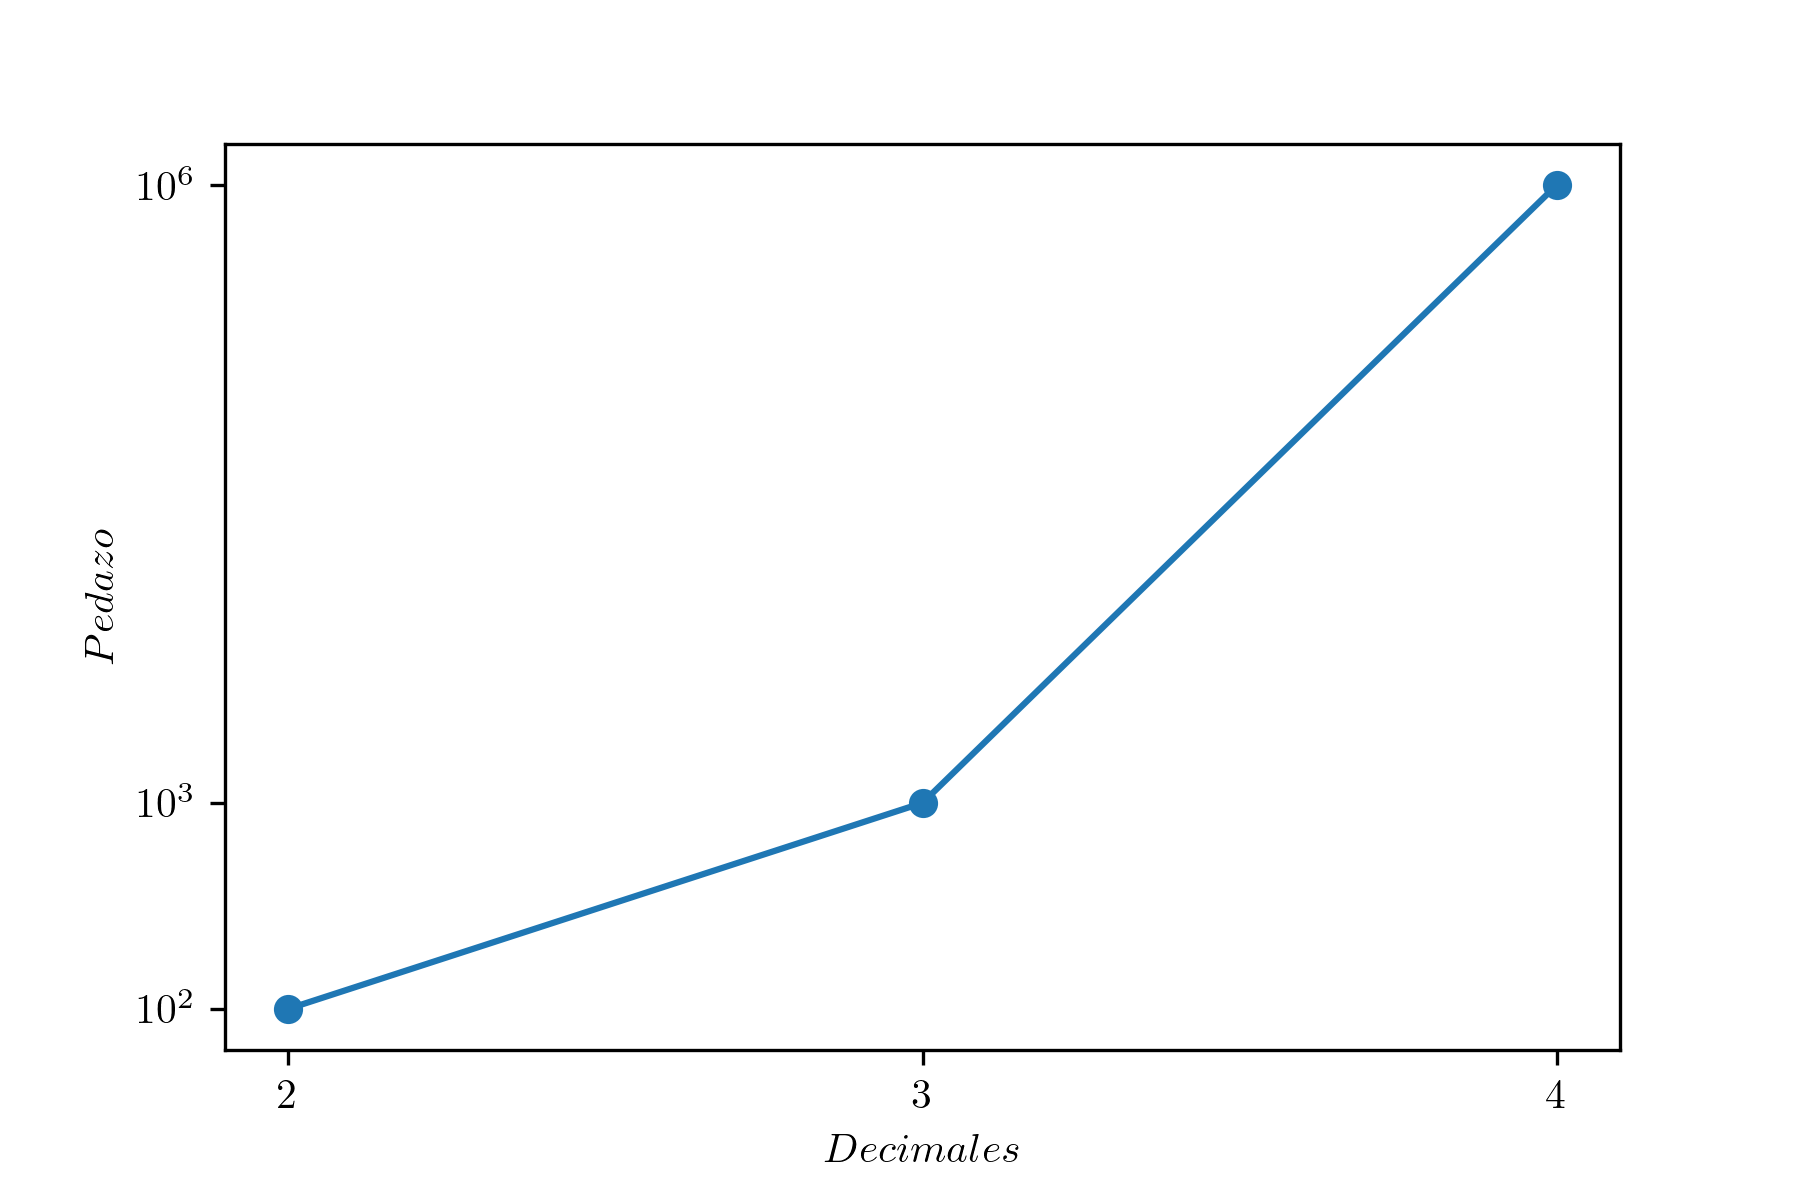
\includegraphics[width=100mm]{p5p1m.png}
\caption{\label{fig3} Gráfica Decimales vs Pedazo.}
\end{figure}

\section{Reto 1}
En este reto se debe de implementar la estimación del valor de de kurt y determinar la relación matemática entre el número de muestras obtenidas y la precisión obtenida en terminos del error absoluto \cite{Satu_Elisa_Schaeffer}.

\renewcommand{\listingscaption}{Código}
\begin{listing}[H]
  \begin{minted}[linenos,mathescape,texcl]{clojure}
runs = 10
cantidad = 1000
er_p = []
d = 0
eti = []
de = []
while runs <= 1000000:
    pi_p = []

    radio = 0.5
    for a in range(cantidad):
        X = np.random.uniform(-radio, radio, runs)
        Y = np.random.uniform(-radio, radio, runs) 
        
        circulo = X**2 + Y**2 <= radio**2
        pi_c = circulo.sum()/ runs * 4
        pi_p.append(pi_c)
    pi_ce = sum(pi_p) / cantidad
    error = abs((pi_ce - pi) / pi_ce) * 100   
    er_p.append(error)
    # print(pi_ce)
    d += 1
    de.append(d)
      \end{minted}
  \label{lst:fibo}
  \caption{Determina la estimación del valor de $\pi$ de kurt.}
\end{listing}
\newpage
En el código anterior calcula $\pi$ usando el método Monte Carlo para esto se usan números aleatorios uniformes \cite{Librería_Reto1} que van desde el radio negativo a positivo, además se calcula el porcentaje absoluto de error cada pedazo de muestra. El código completo se encuentra en GitHub \cite{Denisse_Leyva}.

\begin{figure}[H]
\centering
\begin{subfigure}[b]{0.35\linewidth}
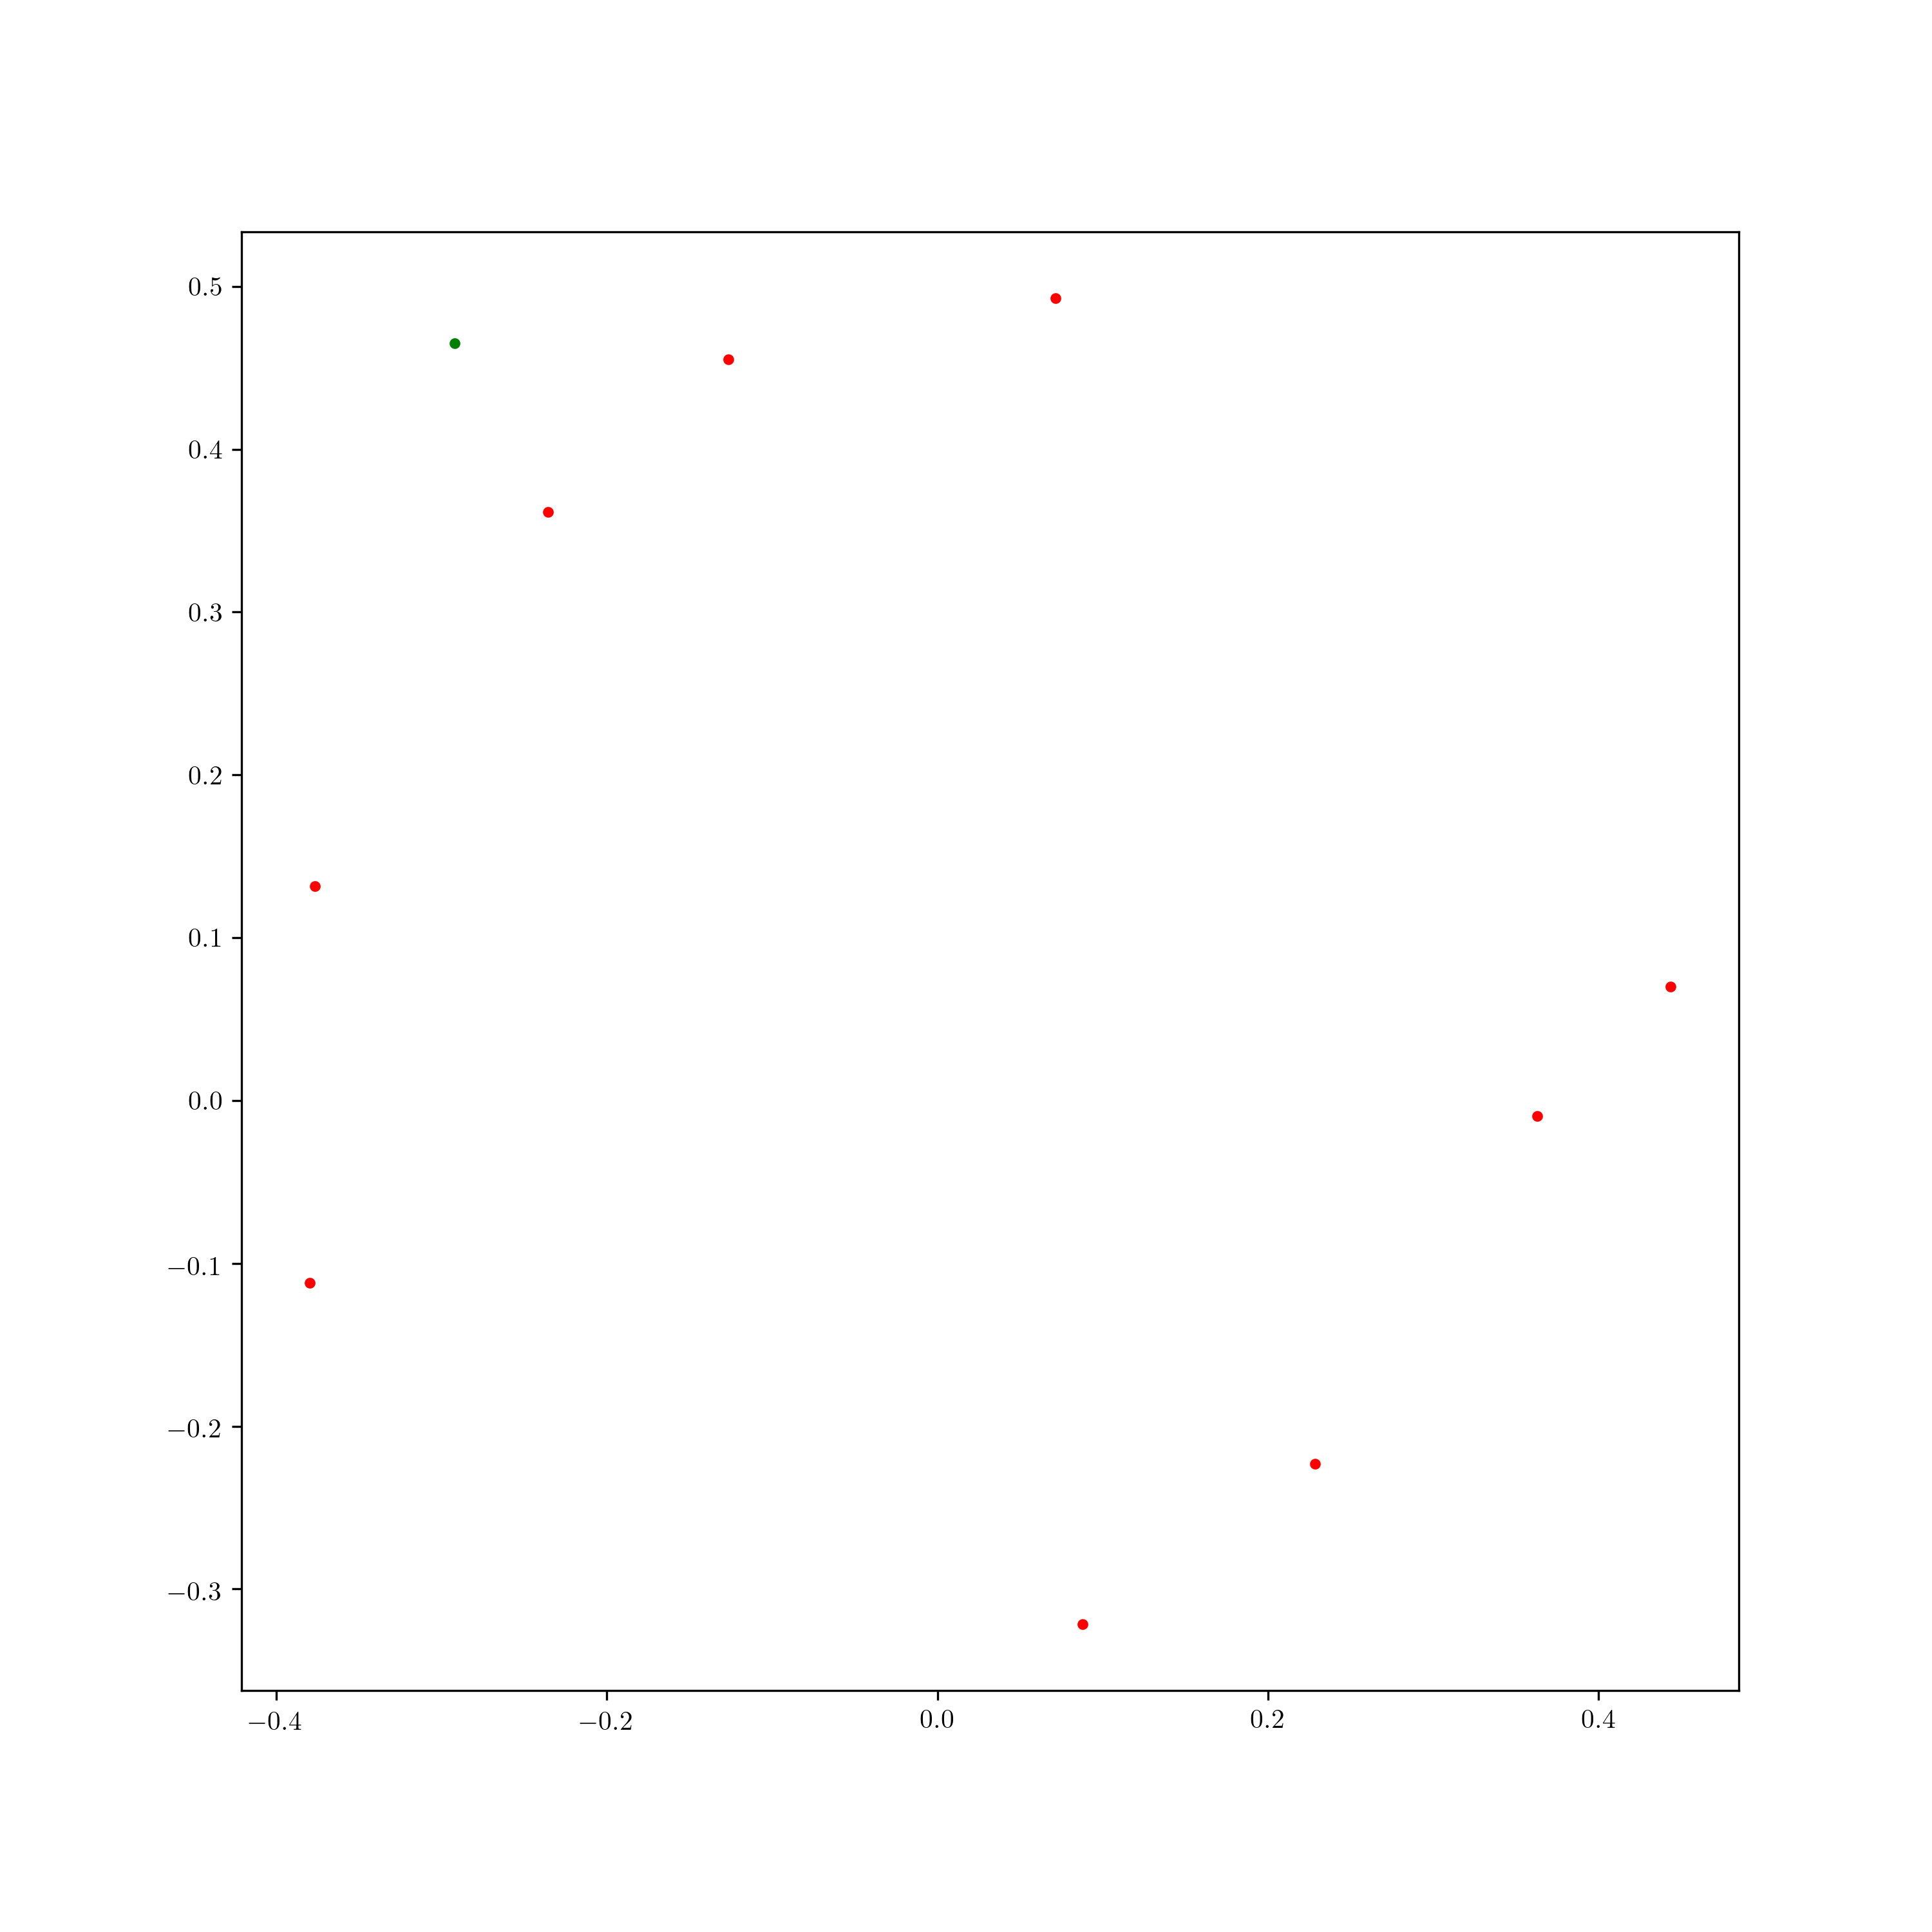
\includegraphics[width=\linewidth]{p5r1f1.png}
\caption{100 muestras estimación\\ de $\pi$ 3.1431.}
\end{subfigure}
\begin{subfigure}[b]{0.35\linewidth}
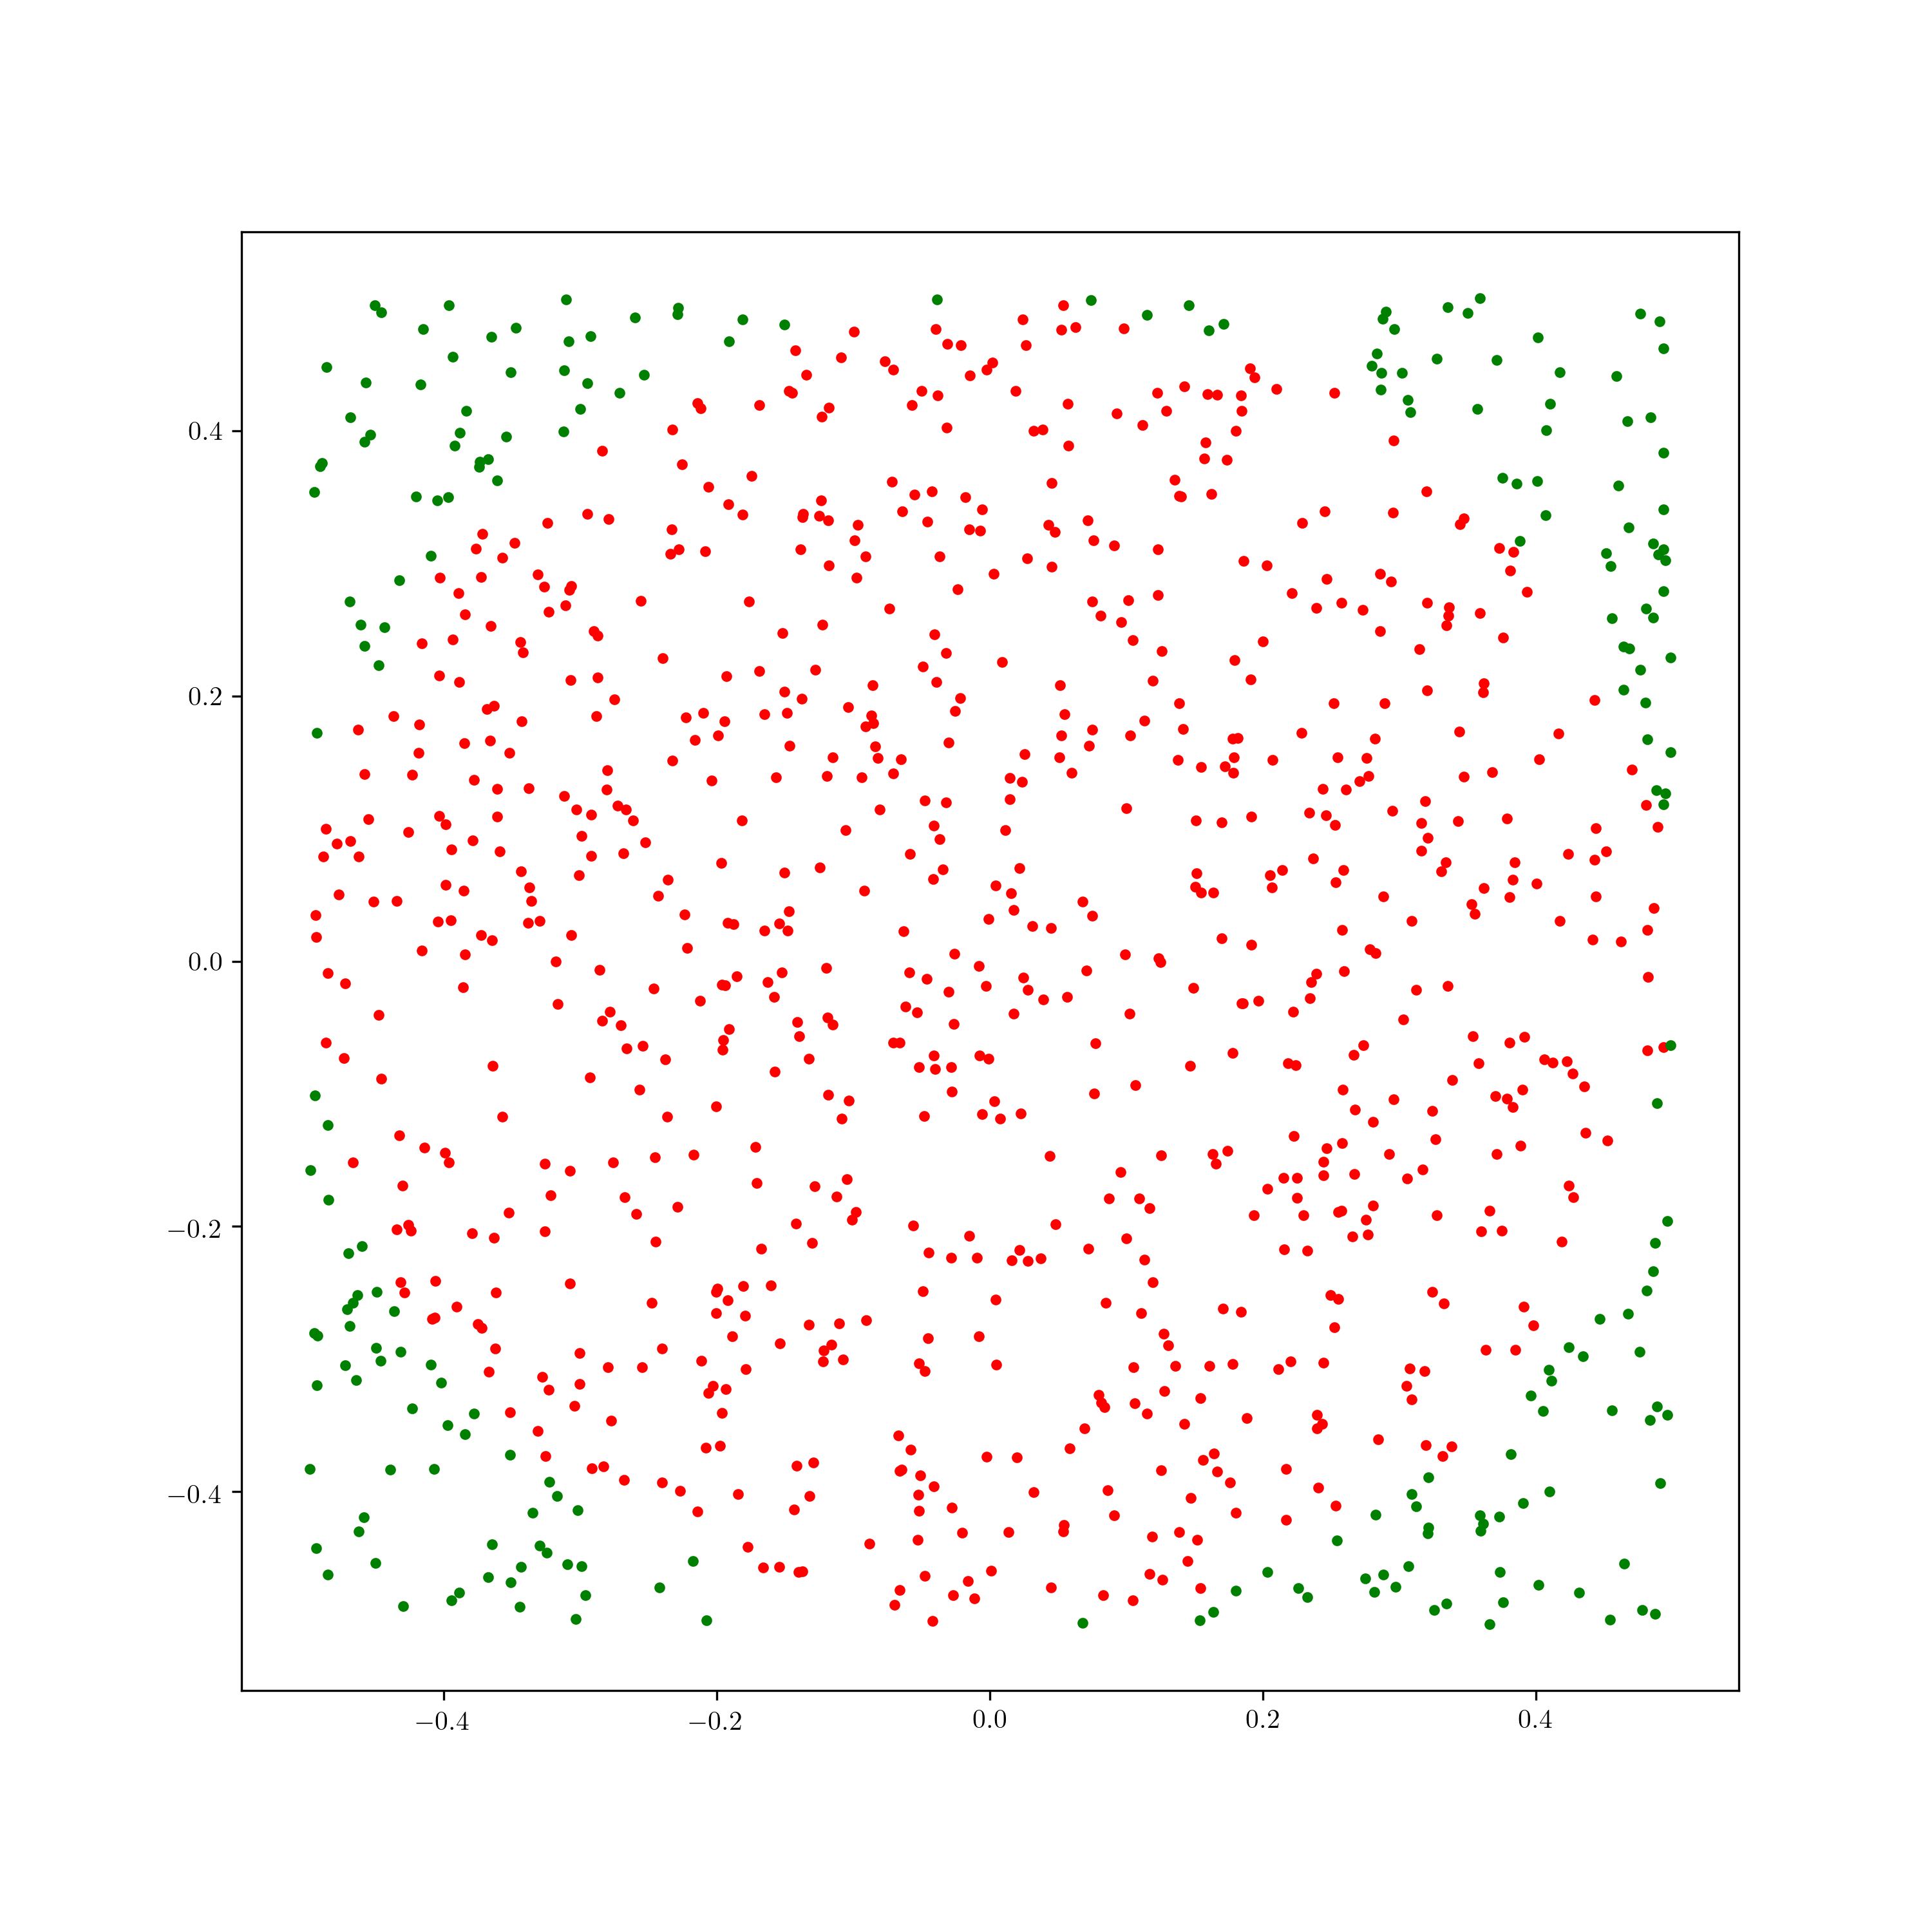
\includegraphics[width=\linewidth]{p5r1f3.png}
\caption{10000 muestras estimación \\ de $\pi$ 3.1418.}
\end{subfigure}
\caption{Imágenes de aproximaxión de $\pi$ con diferente tamaño de muestra.}
\label{fig:westminster}
\end{figure}

\begin{figure}[H]
\centering
\begin{subfigure}[b]{0.35\linewidth}
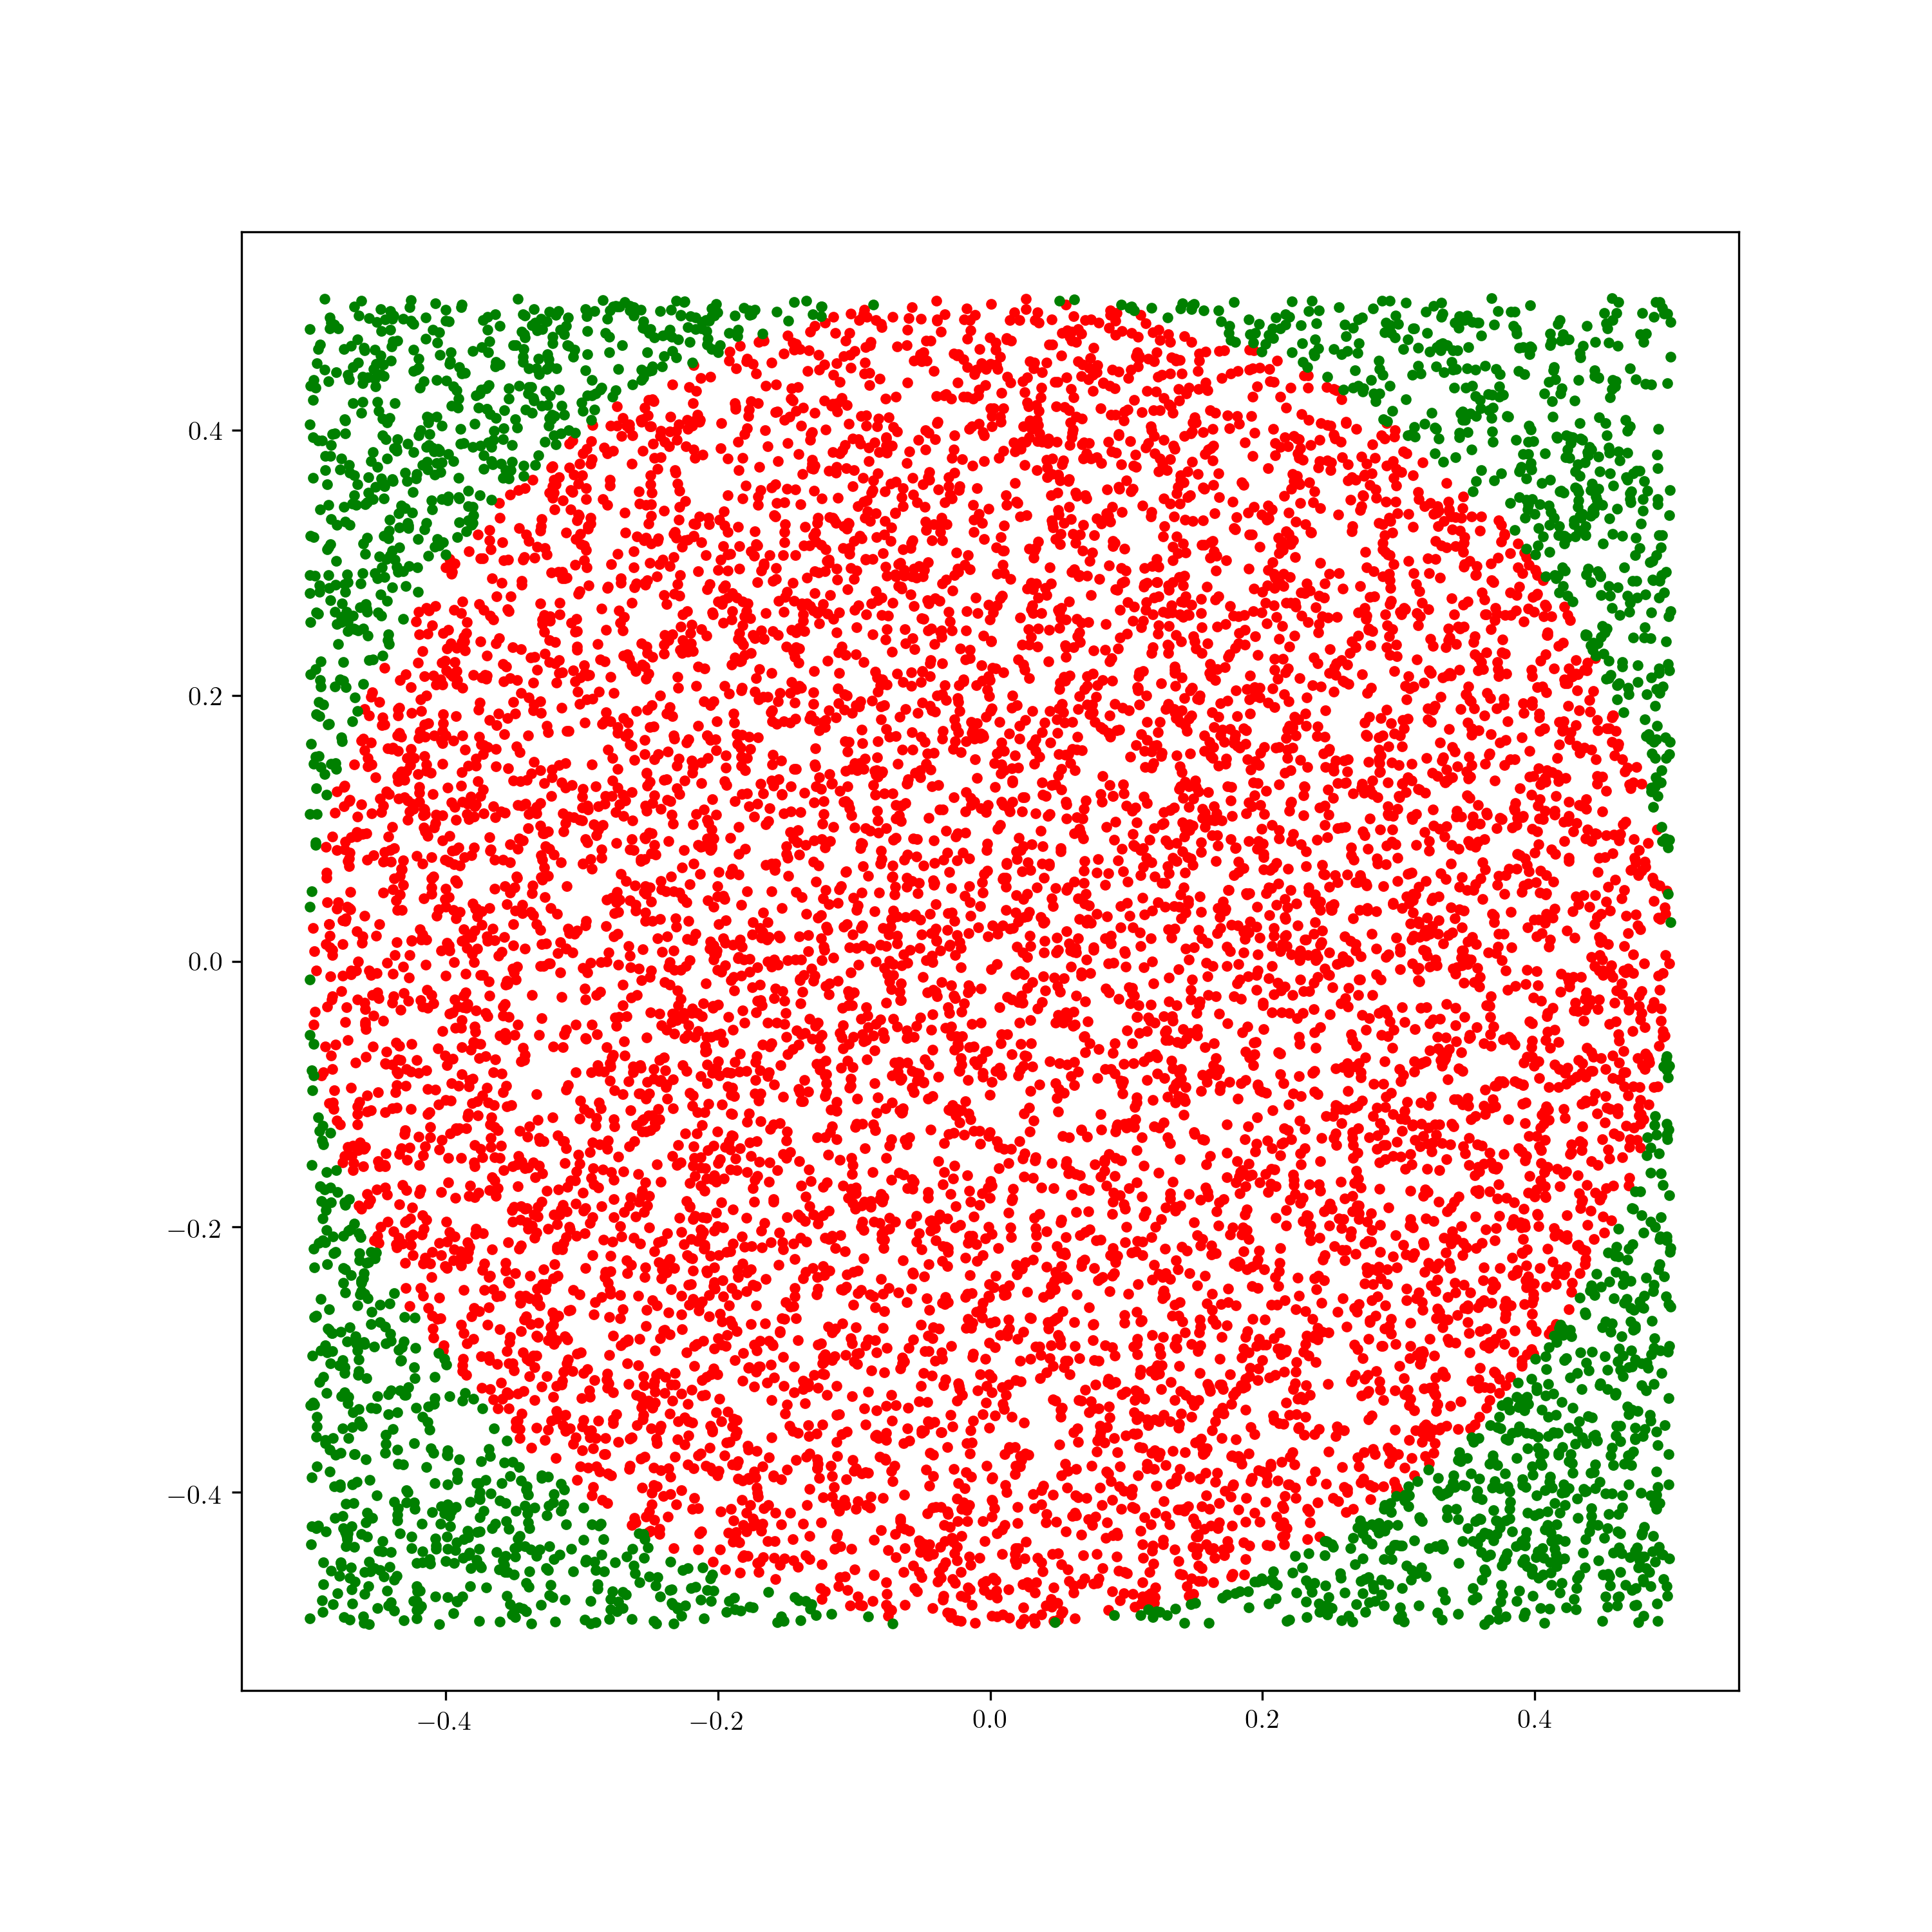
\includegraphics[width=\linewidth]{p5r1f4.png}
\caption{100000 muestras estimación\\ de $\pi$ 3.1426.}
\end{subfigure}
\begin{subfigure}[b]{0.35\linewidth}
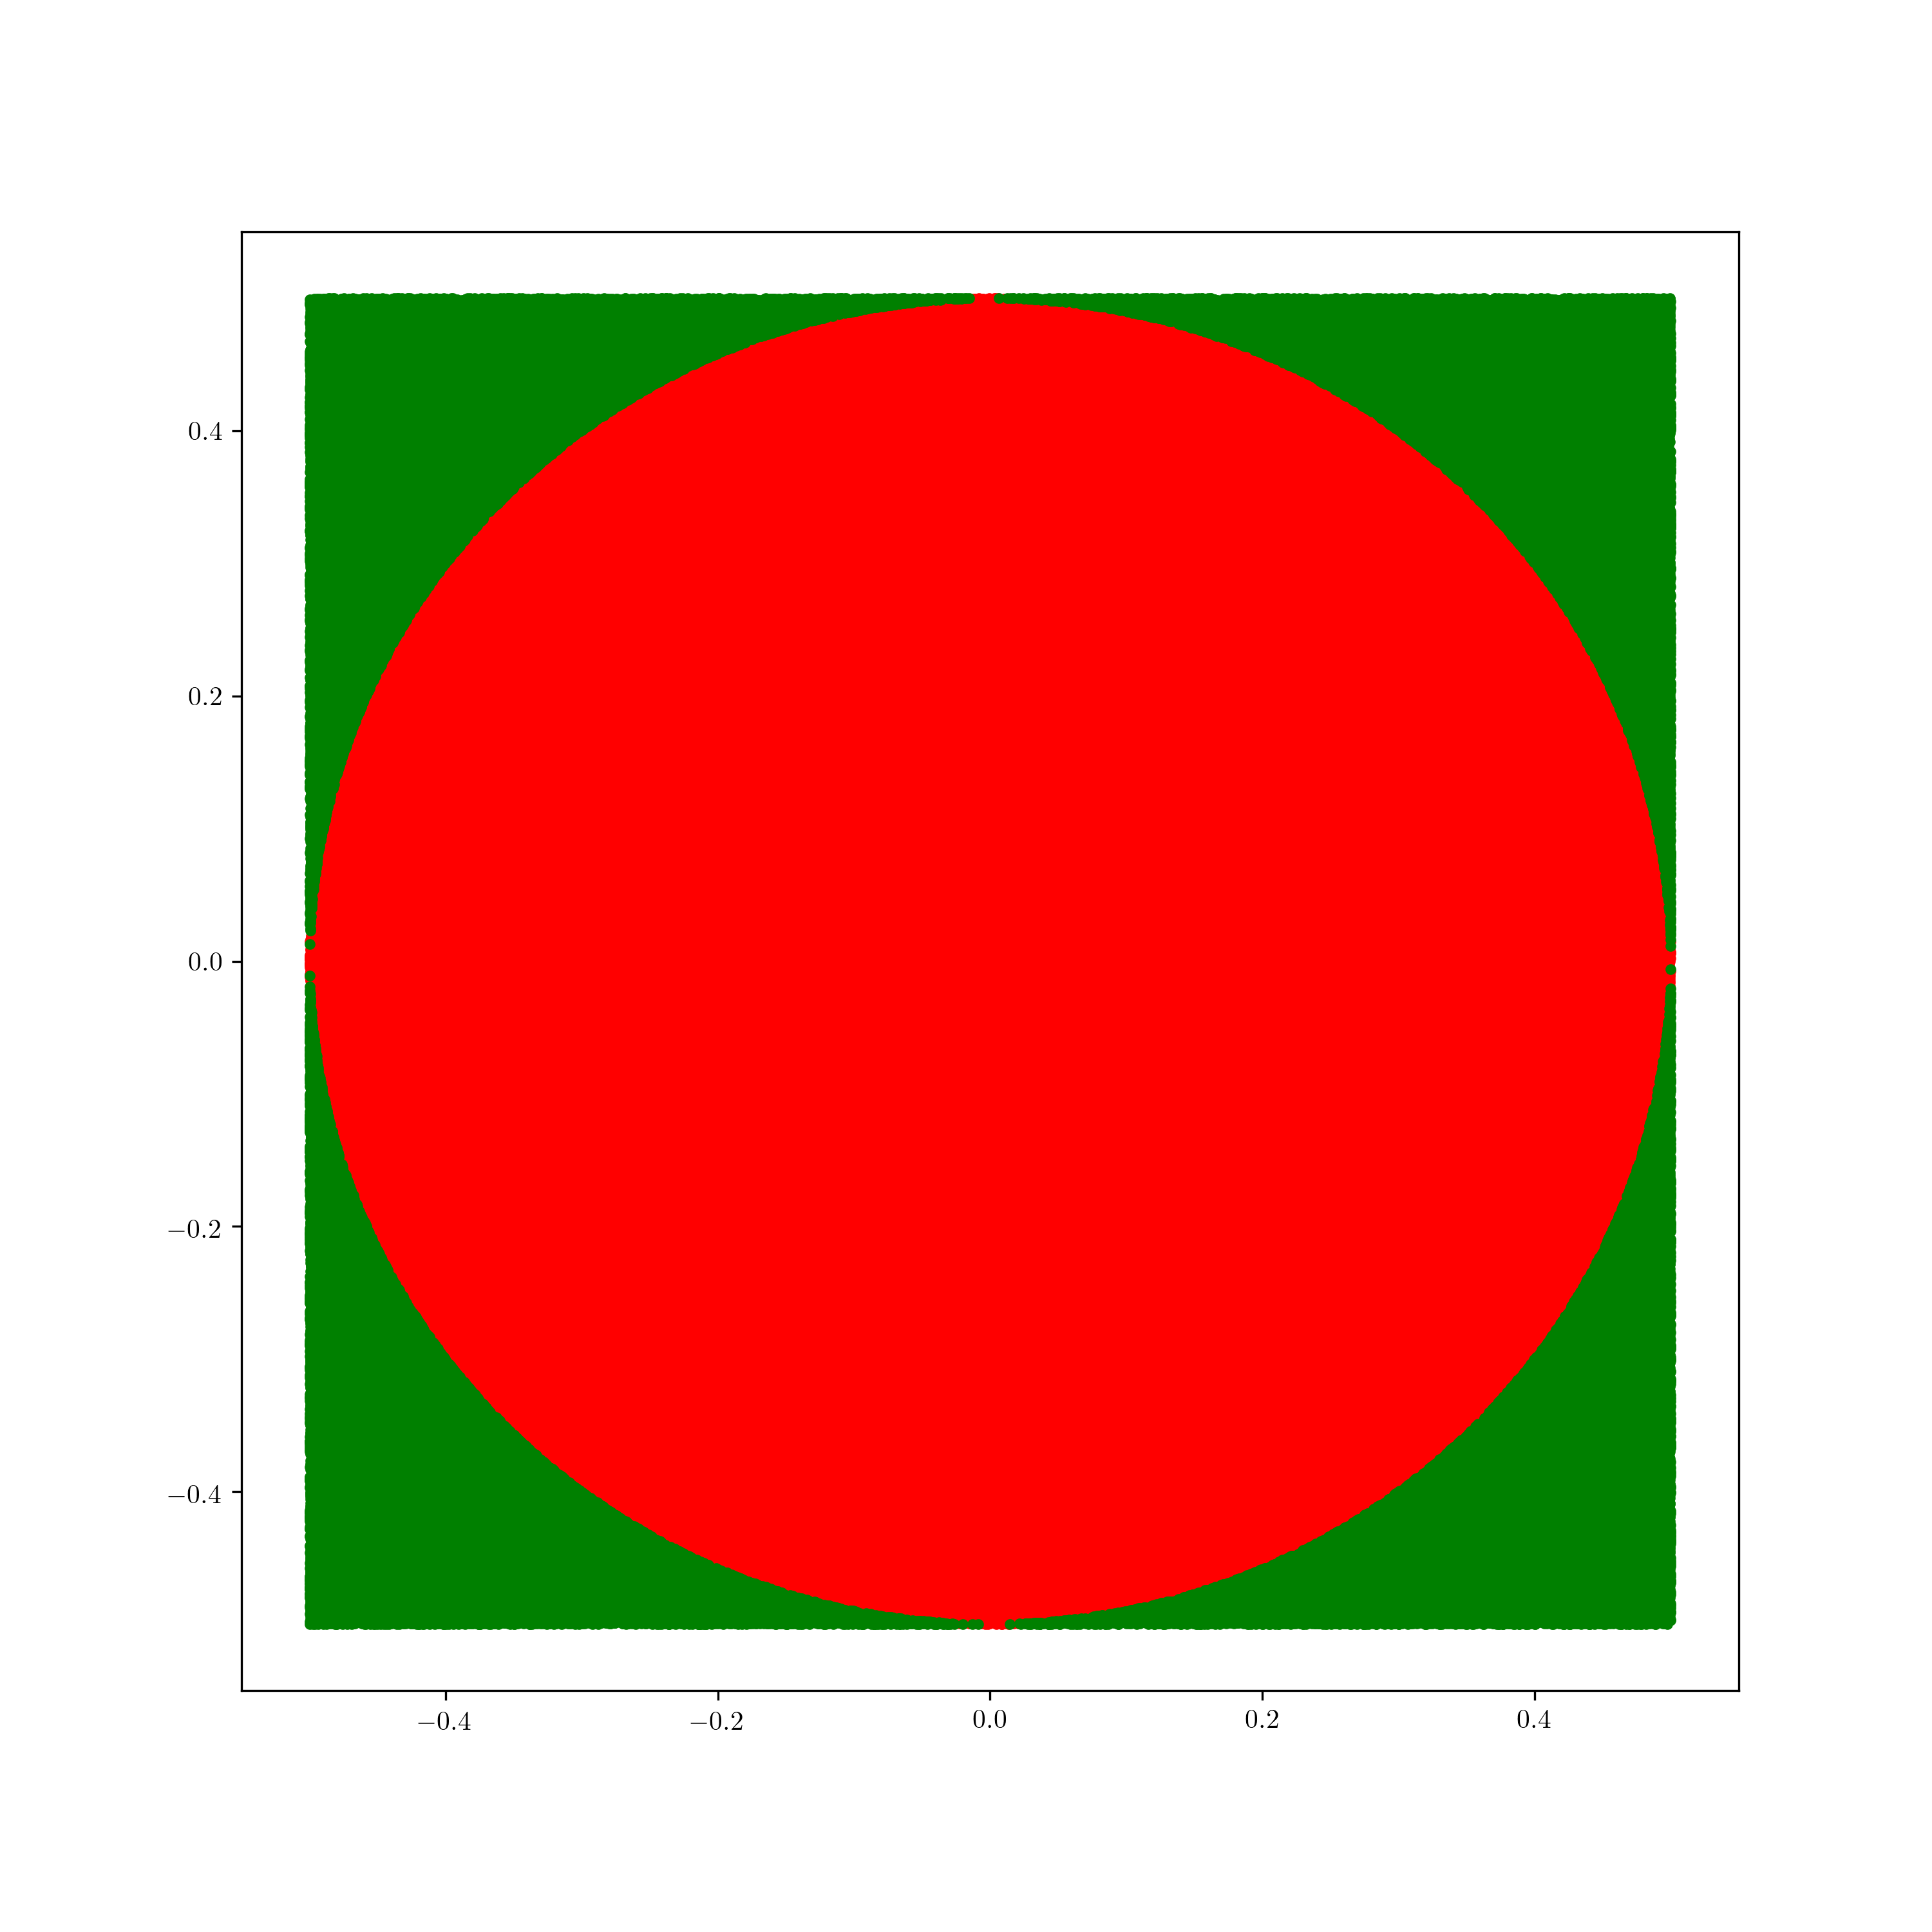
\includegraphics[width=\linewidth]{p5r1f6.png}
\caption{10000000 muestras estimación\\ de $\pi$ 3.1416.}
\end{subfigure}
\caption{Imágenes de aproximaxión de $\pi$ con diferente tamaño de muestra.}
\label{fig:westminster}
\end{figure}

\begin{figure}[H]
\centering
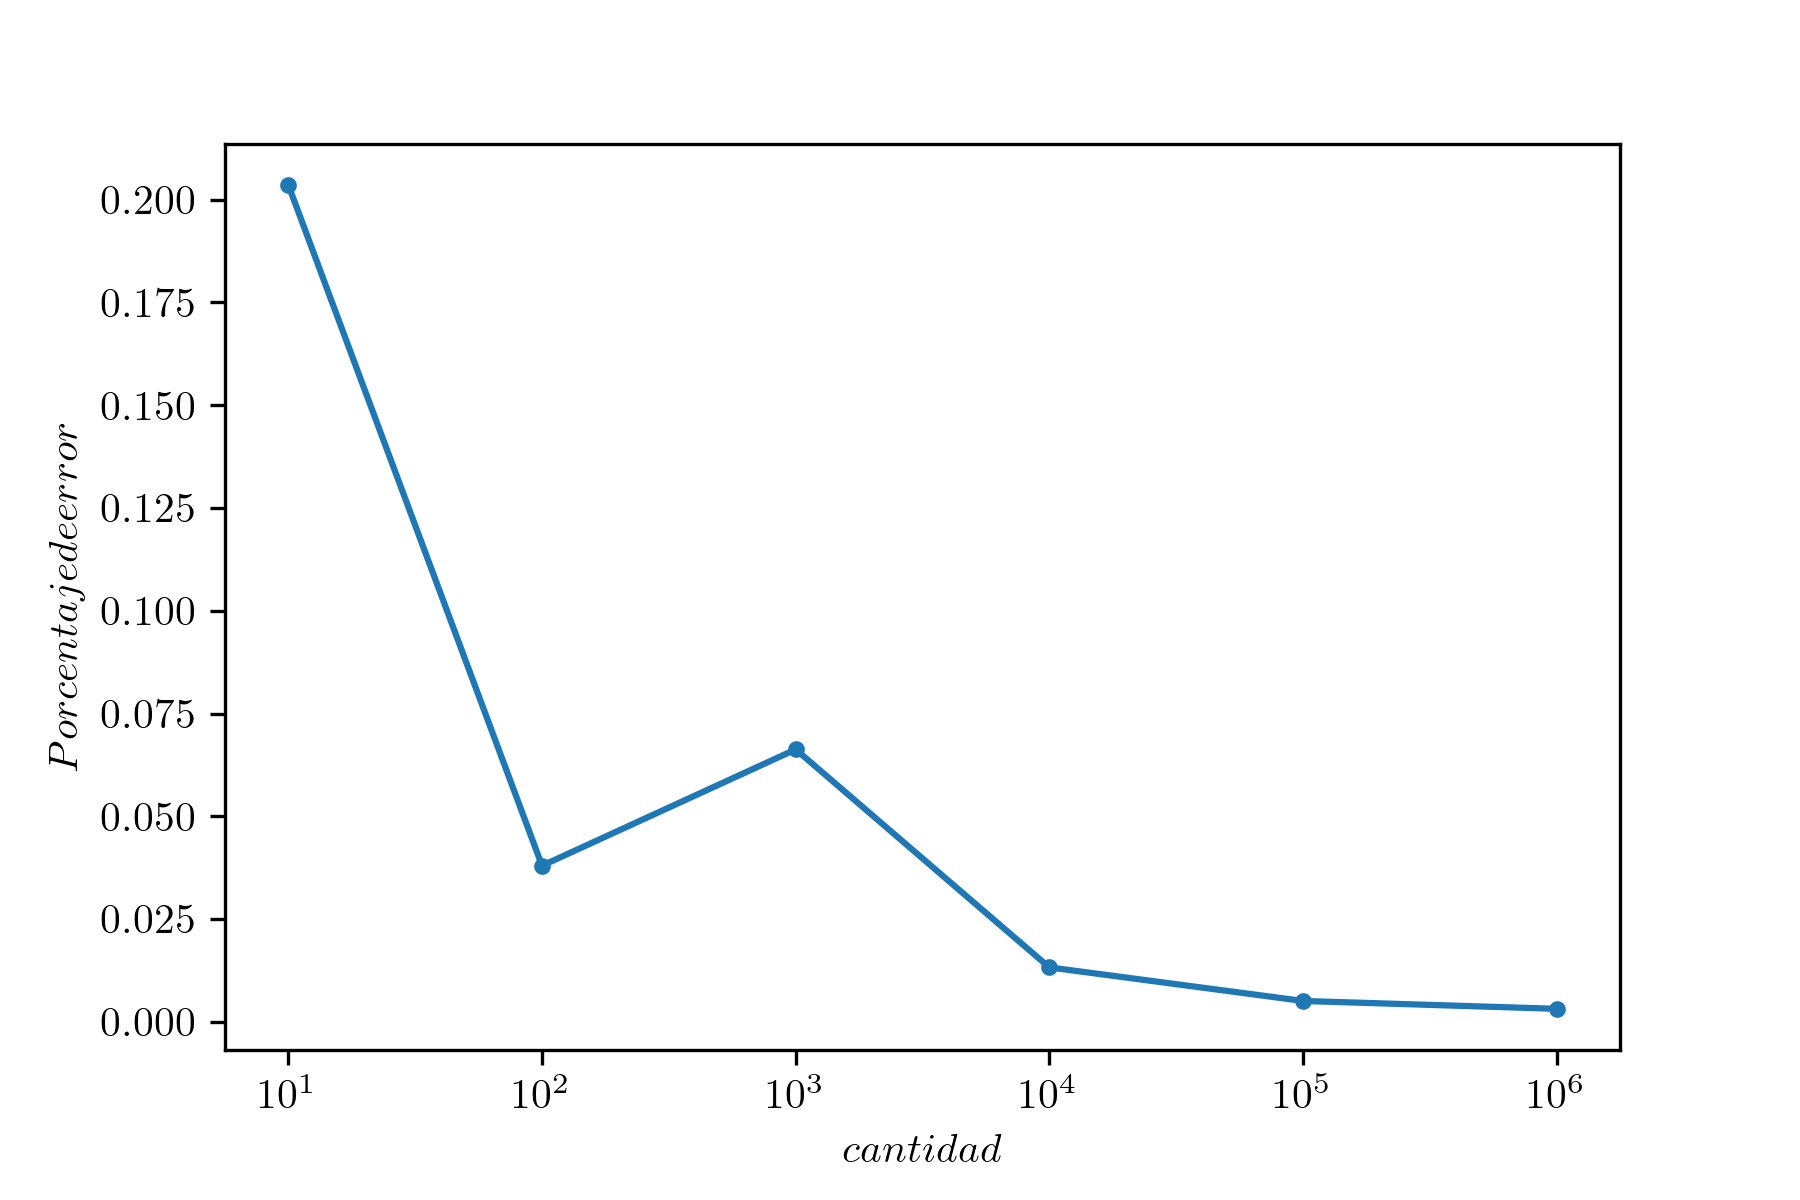
\includegraphics[width=100mm]{p5r1.png}
\caption{\label{fig3} Gráfica de cantidad vs porcentaje de error .}
\end{figure}

Como se puede observar en la gráfica entre mayor cantidad de muestras menor porcentaje de error.

\section{Reto 2}
En este segundo reto se debe aplicar el método Monte Carlo para estimar la cantidad de pintura necesaria en un mural, comparando conteos exactos de pixeles de distintos colores \cite{Satu_Elisa_Schaeffer}. 

\renewcommand{\listingscaption}{Código}
\begin{listing}[H]
  \begin{minted}[linenos,mathescape,texcl]{clojure}
im = Image.open('pera.png')
a = np.asarray(im,dtype=np.float32)/255
plt.figure(figsize=(12,12))
plt.imshow(a)
plt.axis('off')
plt.show()
w, h = im.size
colors = im.getcolors(w * h)
num_colores = len(colors) 
num_pixels = w*h
x, y, z = a.shape
a1 = a.reshape(x*y, z)
n = 10
k_means = KMeans(n_clusters=n)
k_means.fit(a1)
centroides = k_means.cluster_centers_
etiquetas = k_means.labels_
a2 = centroides[etiquetas]
a3 = a2.reshape(x,y,z)
plt.figure(figsize=(12,12))
plt.imshow(a3)
plt.axis('off')
plt.savefig('p5_r2.png', dpi=300)
plt.show()
        \end{minted}
  \label{lst:fibo}
  \caption{Discretiza la imágen.}
\end{listing}

\begin{figure}[H]
\centering
\begin{subfigure}[b]{0.35\linewidth}
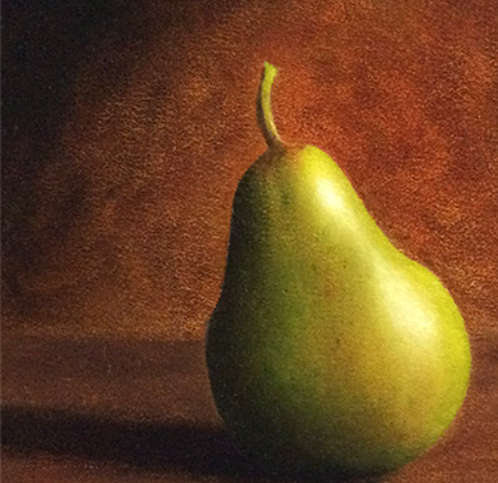
\includegraphics[width=\linewidth]{pera.png}
\caption{Pintura }
\end{subfigure}
\begin{subfigure}[b]{0.35\linewidth}
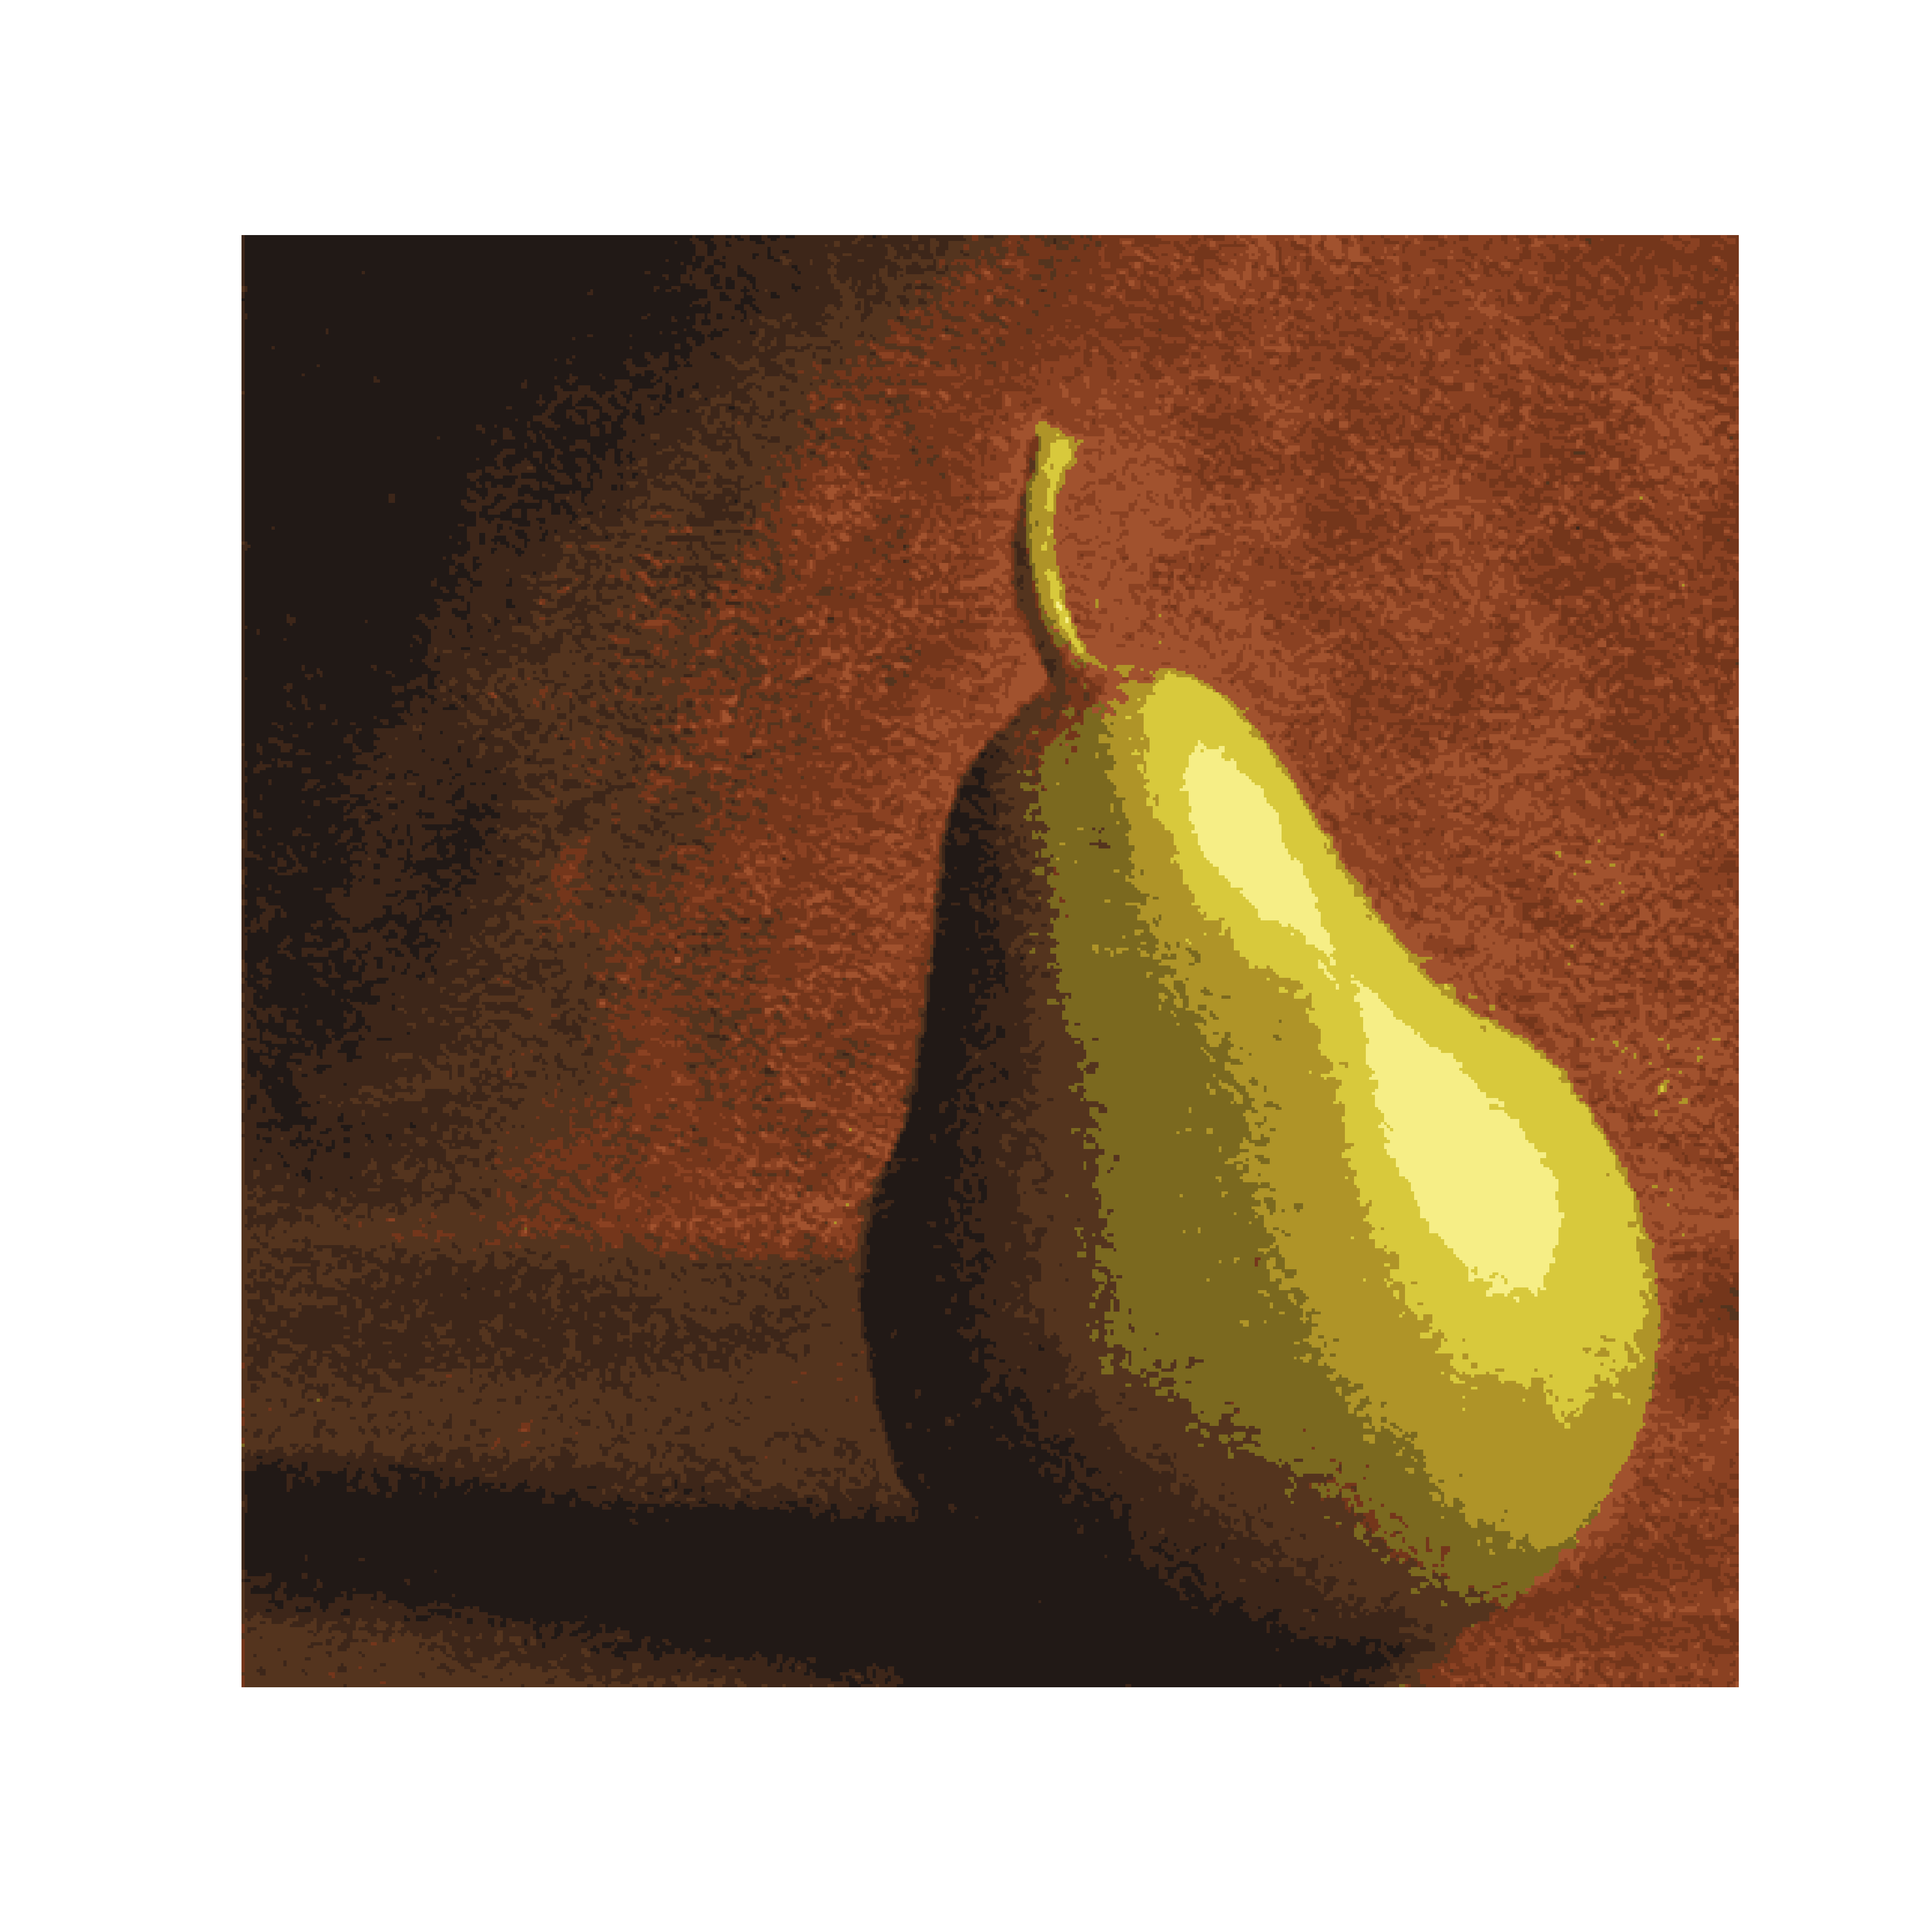
\includegraphics[width=\linewidth]{p5_r2.png}
\caption{Pintura discretizada}
\end{subfigure}
\caption{Imágen original e imágen con un palette de 10 colores.}
\label{fig:westminster}
\end{figure}

\renewcommand{\listingscaption}{Código}
\begin{listing}[H]
  \begin{minted}[linenos,mathescape,texcl]{clojure}
cantidad_c = len(centroides)
porcentajes = [[]]* cantidad_c
litros = [[]] * cantidad_c
colores = [[]] * cantidad_c
for cant in range(cantidad_c):
    X = np.random.uniform(0, h, runs)
    Y = np.random.uniform(0, w, runs) 
    valores = []
    for a in range(runs):
        x = int(X[a])
        y = int(Y[a])
        valores.append(a3[x,y])
       
    porcentaje = []
    for a in range(cantidad_c):
        color = valores == centroides[a]
        suma = color.sum()
        porcentaje.append(((suma-runs)/3)/runs)
        \end{minted}
  \label{lst:fibo}
  \caption{Porcentaje de color que hay en la imágen.}
\end{listing}

\begin{figure}[H]
\centering
\begin{subfigure}[b]{0.40\linewidth}
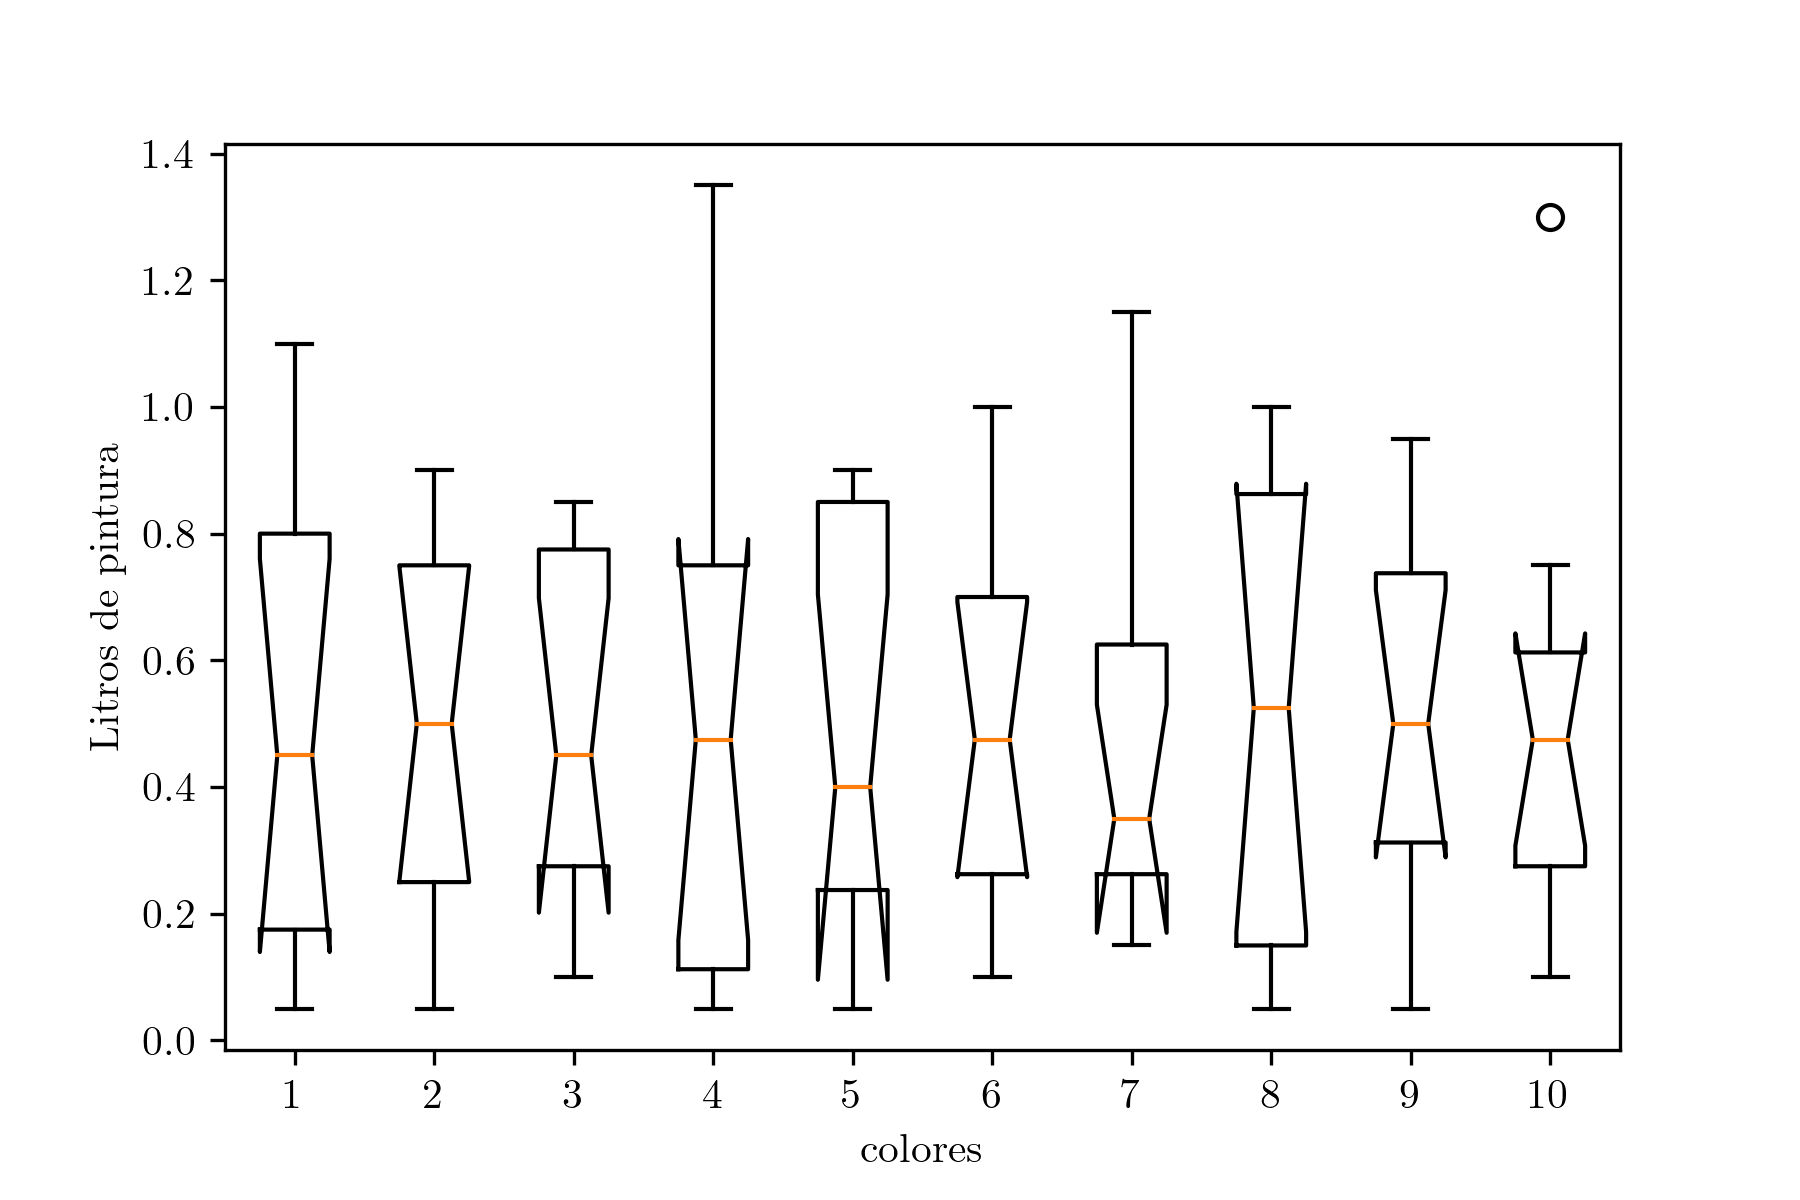
\includegraphics[width=\linewidth]{p5_r2_100.png}
\caption{100 muestras }
\end{subfigure}
\begin{subfigure}[b]{0.40\linewidth}
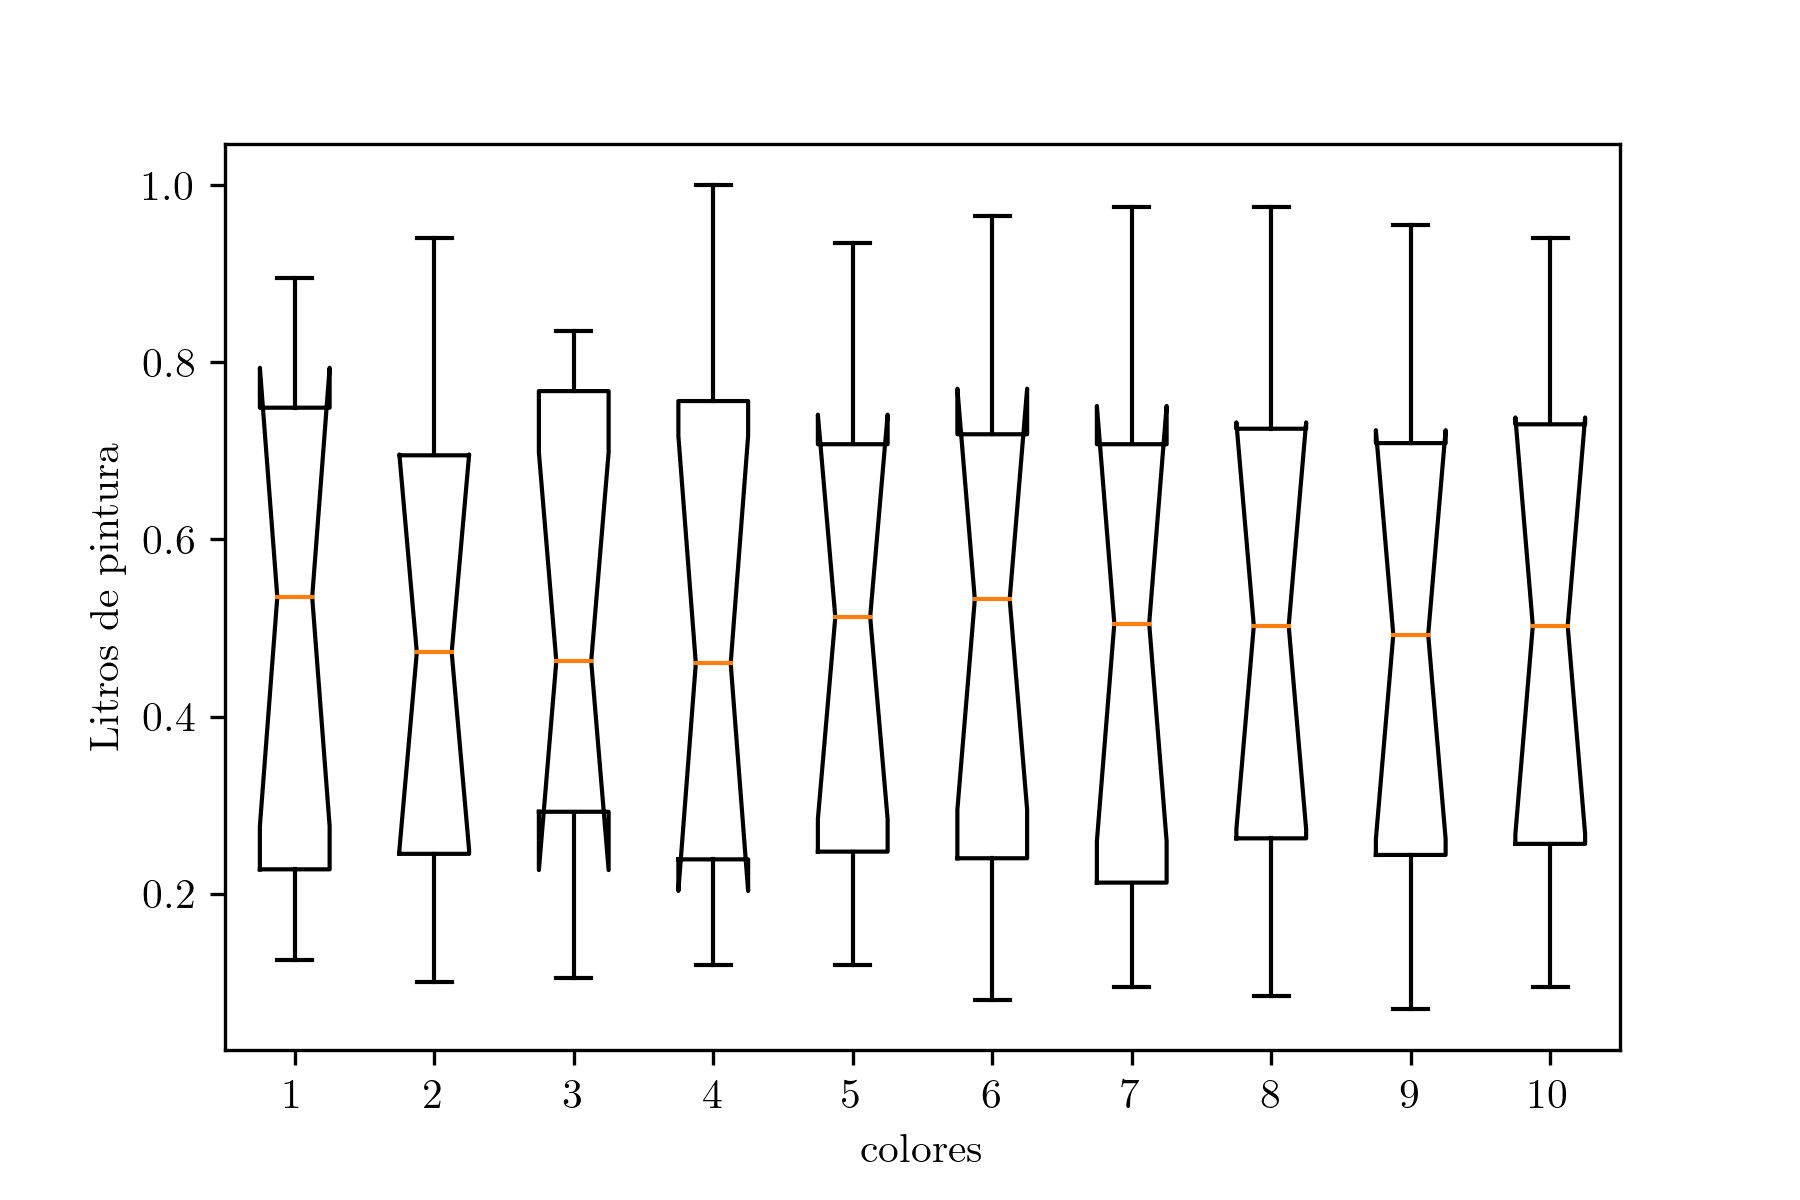
\includegraphics[width=\linewidth]{p5_r2_1000.png}
\caption{1000 muestras}
\end{subfigure}
\caption{Gráfica caja bigote litros de pintura vs colores.}
\label{fig:westminster}
\end{figure}

\begin{figure}[H]
\centering
\begin{subfigure}[b]{0.40\linewidth}
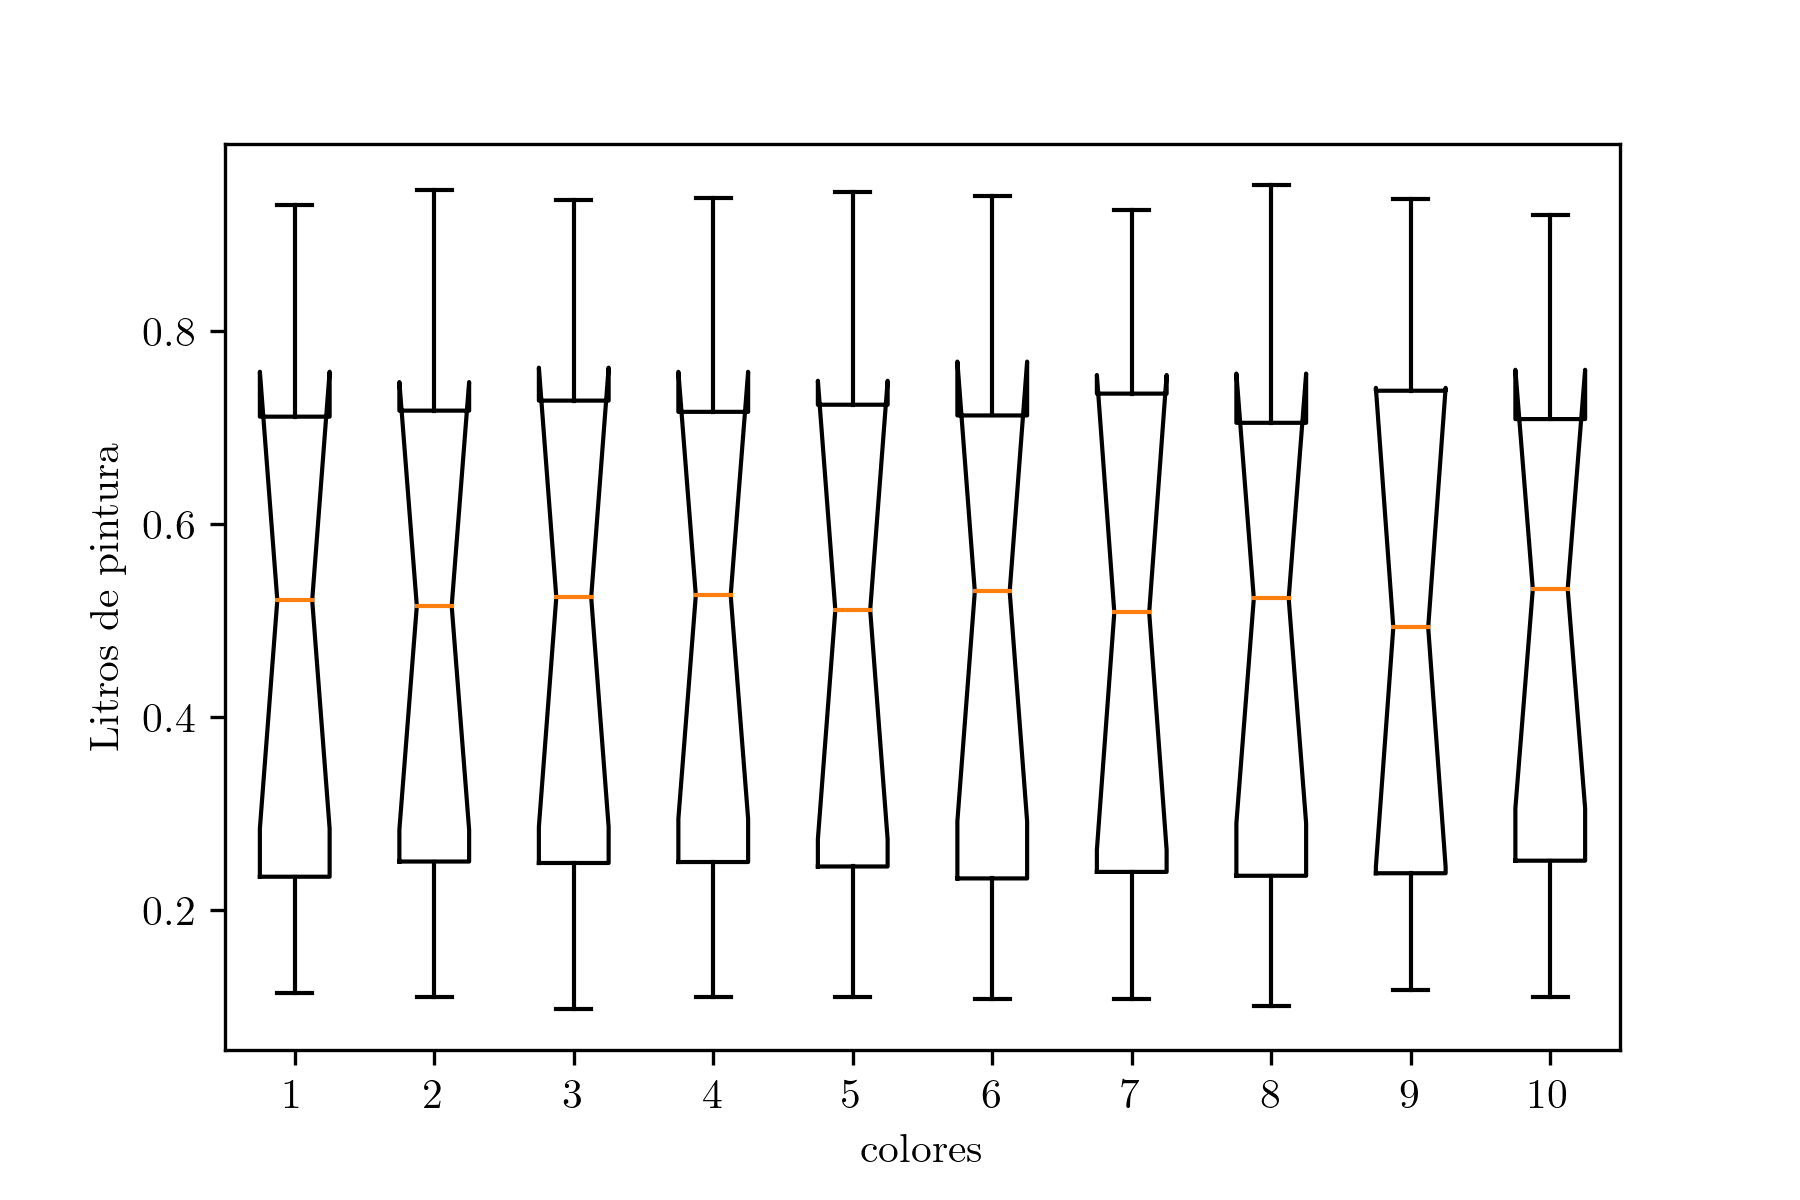
\includegraphics[width=\linewidth]{p5_r2_10000.png}
\caption{10000 muestras }
\end{subfigure}
\begin{subfigure}[b]{0.40\linewidth}
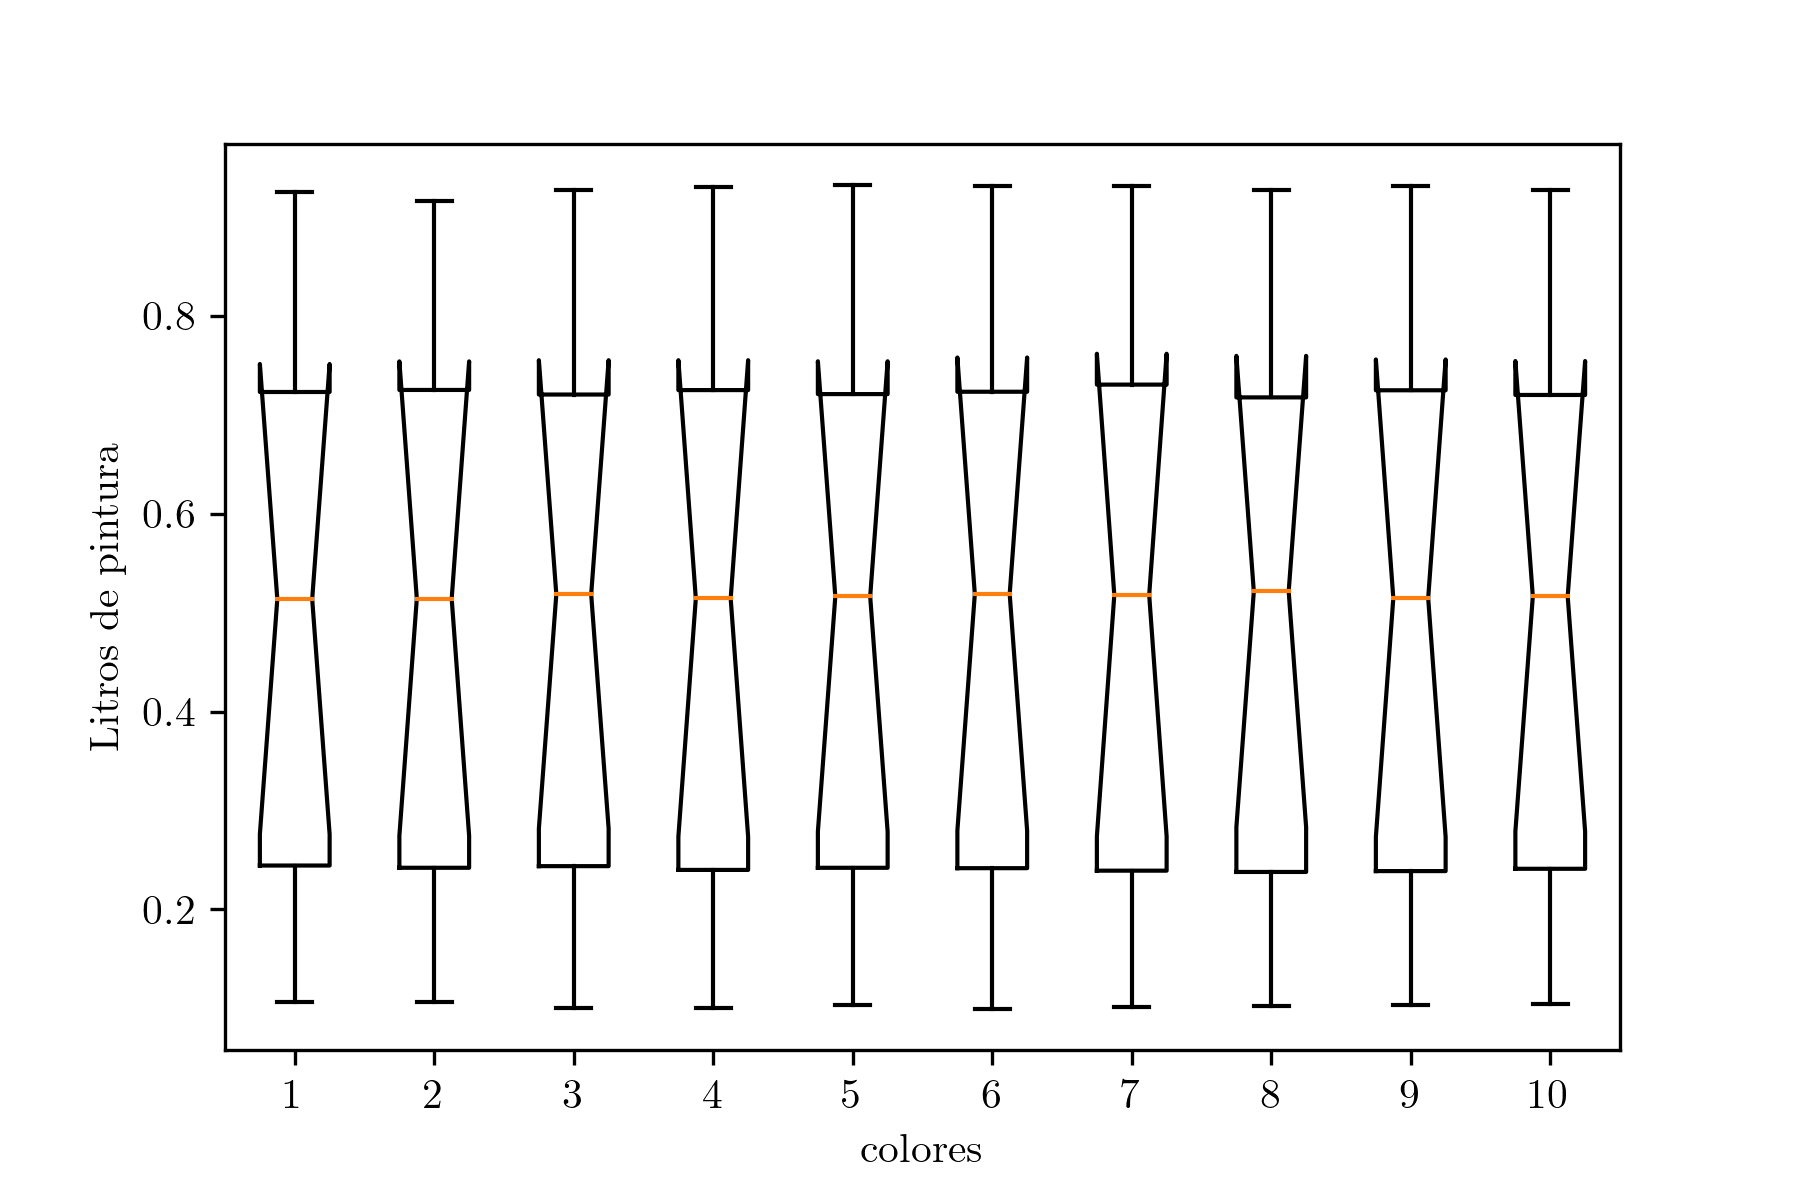
\includegraphics[width=\linewidth]{p5_r2_100000.png}
\caption{100000 muestras}
\end{subfigure}
\caption{Gráfica caja bigote litros de pintura vs colores.}
\label{fig:westminster}
\end{figure}
\printbibliography
\end{document}
